\documentclass[twocolumn]{article}
\usepackage{array,url,kantlipsum}
\usepackage{lmodern}
\usepackage{tikz}
\usepackage{capt-of}
\usepackage{biblatex}
\usepackage{graphicx}
\usepackage{amsmath}
\usepackage{breqn}
\usepackage{rotating}
\usepackage{hyperref}

\addbibresource{paperdyna.bib}

%Tikz initialization
\usetikzlibrary{arrows,decorations.pathmorphing,shapes.geometric}
\tikzset{>=latex}
\tikzset{snake it/.style={decorate, decoration=snake}}
\tikzstyle{startstop} = [rectangle, rounded corners, minimum width=2cm, minimum height=0.5cm,text centered, draw=black]
\tikzstyle{process} = [rectangle, minimum width=3cm, minimum height=0.5cm, text centered, draw=black]
\tikzstyle{decision} = [diamond, minimum width=3cm, minimum height=1.5cm, text width = 2cm, text centered, draw=black]
\tikzstyle{blank} = [circle, minimum width=0.1cm, minimum height=0.1cm, text centered, draw=white]
\tikzstyle{arrow} = [thick,->,>=stealth]



\newcommand{\Mark}[1]{\textsuperscript{#1}}

\begin{document}
\twocolumn[{%
 \centering
 \LARGE Hybrid ARIMA/ANN vs naive model for trading  \\[1.5em]
 \large Repetto Marco\Mark{1},
       \\[1em]
 \normalsize
 \begin{tabular}{*{2}{>{\centering}p{.35\textwidth}}}
  \Mark{1}Dipartimento di Management e Metodi Quantitativi \tabularnewline
  Università degli studi di Milano \tabularnewline
  \url{}marco.repetto@studenti.unimi.it
 \end{tabular}\\[3em] % some more space after the title part
}]

\begin{abstract}
This paper presents the combination of the ARIMA process with ANN. In particular, ARIMA is used to capture the underlying linearities of stock movement whereas the error terms are fed in an ANN given as inputs the price of the stocks from the same market. Such hybrid ARIMA is used for signal generation in the prediction of stock prices movement, especially in such case the goodness of the model is tested in comparison with a naive algorithm that generates signals at random. The portfolio of such game is built using common stocks from NASDAQ and an intraday time series of 90 intervals of one minute each leveraging the Alphavantage API.
\end{abstract}

\section{Introduction}
Trading in securities is probably one of the many fields of finance which saw an incredible automatization over recent years and consequently an improvement in efficiency as well as competition over traders\cite{AvellanedaAlgorithmicHighfrequencytrading2011}.

\begin{figure}
    \centering
    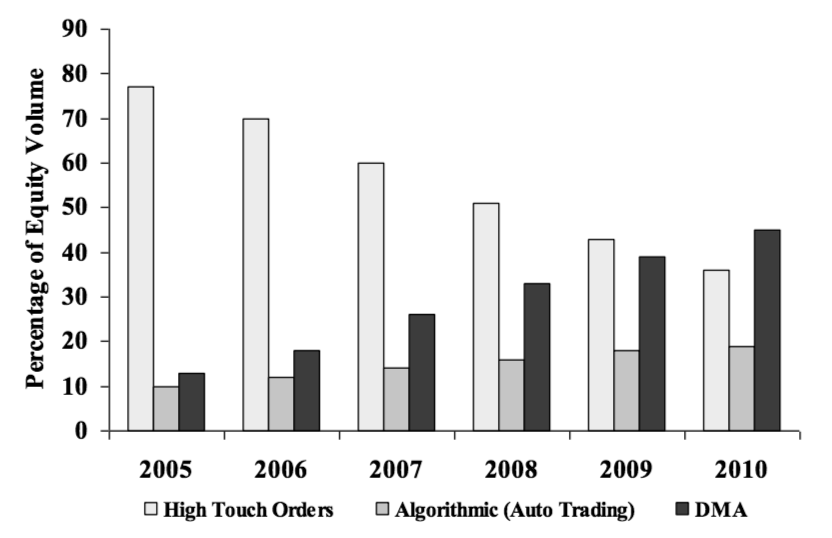
\includegraphics[width=1\linewidth, ]{images/algodata.png}
    \caption{Percentage of order generated by algorithms}
    \label{algodata}
\end{figure}

From this disruptive innovation a completely new professional role came out; the Quant, that is, a professional who is expert in quantitative analysis and in particular in financial modeling. The concept of Quant would not be so important without the concept of algorithmic trading, which is defined as automated trading done by computers which are programmed to take certain actions in response to a variety of market data (or non market data, an example could be tweet sentiment analysis \cite{sul2014trading}). In very simplistic and kind of "naive" words the algorithm take the inputs from the model developed by the Quant and enacts the decision supported by the financial model.
In order to let the algorithm implement market decisions (whether to buy or to sell a particular security) we have to "feed" it with a proper financial model. A typical algorithmic trading process is represented on figure \ref{algoproces}; the overall process consists mainly in 4 cyclical phases where two of them interacts comprehend interactions with the environment, as follows:

\begin{itemize}
\item I phase: consists mainly on data gathering from the environment $E$, in our case, since we are time series model based on stock prices our data will come from the subset $M$ which represent the market data;
\item II phase: at this point the data gathered are used by the professional to create a proper financial model aim at forecast the securities' behavior under scope; 
\item III phase: this phase embrace the activities of back-testing of the financial model built by the professional;
\item IV phase: eventually the financial model is deployed and starts to interact with the market $M$, buying and selling a specific securities.
\end{itemize}

In this paper, we decided to operate a un interval horizon forecast using a model based on time series, precisely an ARIMA (Auto Regressive Integrated Moving Average) process. Plus following what reported by Zhang et al.\cite{zhang_time_2003} we associated the ARIMA process with an Artificial Neural Network set to capture the behavior of the fitting errors of the ARIMA process we built previously. The neural net has as inputs current stock prices, conversely on what proposed by Zhang that set as inputs the previous fitting errors. The reason behind this choice is rather simple, whether the ARIMA process is good at capturing the linear behavior of our time series this not happens in case of some nonlinearities that may be well fitted by an ANN. Plus we would like to validate whether the behavior of the stocks under scope is affected by the price behavior of other stocks constituting the portfolio.
In doing so, we defined an algorithm for a pseudo-real-time signal generation. Based on such signal the algorithm enacts the decision whether to buy a stock (forecasting its increase in price) or sell it (because the price will fall in the next interval). In order to measure the goodness of such algorithm, we let it compete with a "naive" algorithm that performs buy and sell decision at random. We measure the aggregate profit and loss for every stock we tested and we built a set of confusion matrix to measure the signal accuracy.

\begin{center}
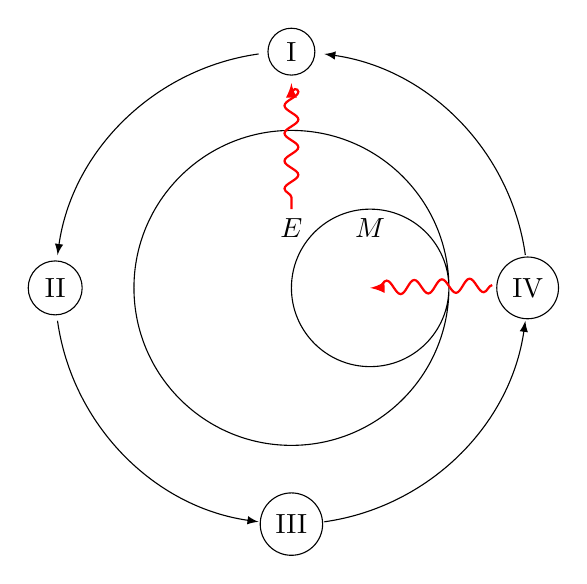
\begin{tikzpicture}

\def \n {4}
\def \radius {3cm}
\def \margin {8} % margin in angles, depends on the radius

  \node[draw, circle] at ({360/\n * (1 - 1)}:\radius) {IV};
  \draw[->, >=latex] ({360/\n * (1 - 1)+\margin}:\radius) 
    arc ({360/\n * (1 - 1)+\margin}:{360/\n * (1)-\margin}:\radius);
    
     \node[draw, circle] at ({360/\n * (2 - 1)}:\radius) {I};
  \draw[->, >=latex] ({360/\n * (2 - 1)+\margin}:\radius) 
    arc ({360/\n * (2 - 1)+\margin}:{360/\n * (2)-\margin}:\radius);
    
     \node[draw, circle] at ({360/\n * (3 - 1)}:\radius) {II};
  \draw[->, >=latex] ({360/\n * (3 - 1)+\margin}:\radius) 
    arc ({360/\n * (3 - 1)+\margin}:{360/\n * (3)-\margin}:\radius);
    
     \node[draw, circle] at ({360/\n * (4 - 1)}:\radius) {III};
  \draw[->, >=latex] ({360/\n * (4 - 1)+\margin}:\radius) 
    arc ({360/\n * (4 - 1)+\margin}:{360/\n * (4)-\margin}:\radius);


\draw (0,0) circle (2) (0,1)  node [text=black,below] {$E$}
      (1,0) circle (1) (1,1)  node [text=black,below] {$M$};
\path [->, thick,draw=red,snake it]
    ({360/5 * (0.9 - 1)+\margin}:2.55) -- (1,0);
\path [<-, thick,draw=red,snake it]
    ({(360/\n * (2 - 1))}:2.6) -- (0,1);
%\draw[draw=blue, snake it] (2,0) arc (0:180:2cm);

\end{tikzpicture}
\end{center}
\captionof{figure}{Algorithmic trading process}
\label{algoproces}


\subsection{AutoRegressive Integrated Moving Average: key concepts and features}
ARIMA processes are a class of univariate time series models, this kind of models attempt to predict financial variables using only information contained in their own past values and possibly current and past values of an error term. ARIMA process differs from the exponential smoothing since ARIMA focuses on the autocorrelation of the time series instead of trend and seasonality. Such model firstly proposed by Box-Jenkins\cite{BoxGeorgeTimeSeriesAnalysis} combines three factors, namely: differencing, autoregressive model and moving average model.
\bigbreak
Where differencing is intend as the process of transformation of the time series such that we end up with a stationary time series which has as main property no time dependency, in other terms given $X_t$ a stochastic process and $F_X(x_{t_k+\theta})$ its cumulative distribution. $X_t$ is stationary when; $\forall k,\theta and t_k$ we have that:
\[ F_x(x_{t_{k+\theta}}) = F_x(x_{t_k}) \]
Autoregressive models are instead defined as:
\[ c+\phi_1L+...+\phi_pL^p+\epsilon_t \]
In this models, we try to forecast future values using a linear combination of past values.
A different approach is taken by moving average processes since they do not use past values but instead a regression of the forecast errors.
Moving average models are defined as:
\[c + (\theta_1 L + ... + \theta_q L^q)\epsilon_t \]
The concatenation of the three gives us the ARIMA process obtained as:

\resizebox{0.90\hsize}{!}{
$
 \underbrace{1-\phi_1L-...-\phi_pL^p}_{AR(p)} + \underbrace{(1-L)^d y_t}_{Differencing(d)} + \underbrace{c + (1 + \theta_1 L + ... + \theta_q L^q)\epsilon_t}_{MA(q)}
$}
In setting such model we used the \textit{forecast} package provided in R \cite{RobHyndmanForecastpackage}
and especially we used the \textit{auto.arima} function to establish the proper ARIMA for each time series. The algorithm is set in a way that let the machine figure out the best model to apply to the specific time series, choosing the right $(p,d,q)$ coefficients. The process is two-tiered: \cite{hyndman_automatic_2007}:
\begin{itemize}
    \item Step 1: start with four possible models
    \item Step 2: consider up to thirteen variations on the current model
\end{itemize}
When a model score a lower AIC than the current one the new model become the current one and the procedure is repeated until the solution converges to the current model. In doing so some constraints are applied by default in order to reach the best solution in a reasonable amount of time.


\subsection{Artificial Neural Network}
The concept of Artificial Neural Network was firstly proposed by Warren S. McCulloch \cite{mcculloch_logical_1943}.
After a period of stagnation caused by the low processing power of computers at that time, the field saw an incredible expansion in our days and its researching community is one of the most active and perhaps flourish that existed so far.
An Artificial Neural Network is a net based on a series of elements called neurons that are represented by an activation function that given a certain number of inputs will return an output based on the weights it has.Such activation functions may vary but they are all linear as firstly proposed by B. Widrow \cite{b._widrow_et_al._adaptive_}.
Fundamental for an artificial neural network is the number of hidden layers that compose such network which may vary from 1 to $n$. In our case, we used an artificial neural network with just one hidden layer as proposed by the diagram in figure 3.
\\
The main advantages of neural networks are their ability of capture the nonlinear relationship in the data (because of this they are addressed as a universal function approximator). However, this ability as a flexibility poses a serious threat to its usage, since they tend to over-fit the data and therefore they may be not best suited for long-run forecasting\cite{rud_data_2001}.

\tikzset{%
  every neuron/.style={
    circle,
    draw,
    minimum size=0.5cm
  },
  neuron missing/.style={
    draw=none, 
    scale=4,
    text height=0.333cm,
    execute at begin node=\color{black}$\vdots$
  },
}

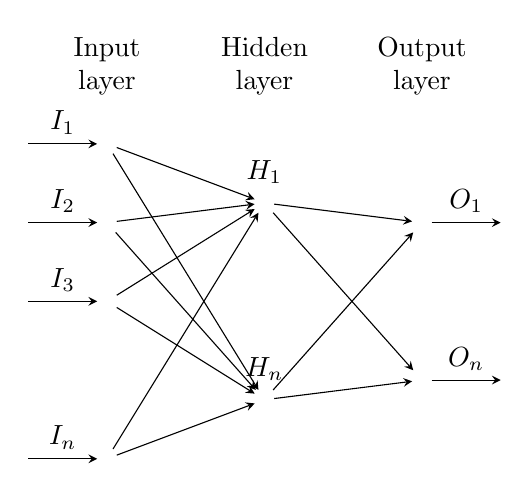
\begin{tikzpicture}[x=1cm, y=1cm, >=stealth]

\foreach \m/\l [count=\y] in {1,2,3,missing,4}
  \node [every neuron/.try, neuron \m/.try] (input-\m) at (0,2.5-\y) {};

\foreach \m [count=\y] in {1,missing,2}
  \node [every neuron/.try, neuron \m/.try ] (hidden-\m) at (2,2-\y*1.25) {};

\foreach \m [count=\y] in {1,missing,2}
  \node [every neuron/.try, neuron \m/.try ] (output-\m) at (4,1.5-\y) {};

\foreach \l [count=\i] in {1,2,3,n}
  \draw [<-] (input-\i) -- ++(-1,0)
    node [above, midway] {$I_\l$};

\foreach \l [count=\i] in {1,n}
  \node [above] at (hidden-\i.north) {$H_\l$};

\foreach \l [count=\i] in {1,n}
  \draw [->] (output-\i) -- ++(1,0)
    node [above, midway] {$O_\l$};

\foreach \i in {1,...,4}
  \foreach \j in {1,...,2}
    \draw [->] (input-\i) -- (hidden-\j);

\foreach \i in {1,...,2}
  \foreach \j in {1,...,2}
    \draw [->] (hidden-\i) -- (output-\j);

\foreach \l [count=\x from 0] in {Input, Hidden, Output}
  \node [align=center, above] at (\x*2,2) {\l \\ layer};

\end{tikzpicture}
\captionof{figure}{Artificial Neural Network scheme}
\label{neural net}

Even though the structure may seem simple one hidden layer ANN reveled to be incredibly reliable on specific task, plus they carry with them greater speed of computation because of its simplicity\cite{the_international_neural_network_society_inns_the_ieee_neural_network_council_cooperating_societies_multi-layer_1990}. As a rule of thumb we take what proposed by Hayashi et al. "Never try a multilayer model for fitting data untill you have tried a single-layer model". Unfortunately there's not such rule of thumb that may help in case of chosing the number of neurons per layer but we choose a number equal two thirds the number of input. 

\newpage

\subsection{Hybrid ARIMA/ANN process}

As mentioned previously the ARIMA process is better suited to capture the linearities of a stochastic process, but what about its nonlinearities? How can we capture them in order to get a better result in our prediction?
An attempt to overcome this problem could be the mixture of some other methods that are built to track such patterns. This is the reason why we chose the hybrid model ARIMA/ANN to do this job.
The mixed-use of ARIMA and neural networks was firstly made by P. Zhang.
Such process compared to the plain vanilla ARIMA has the advantage of capture features that are not modeled by a univariate process like the ARIMA. In our case, we use the neural networks to capture the fitting error behavior of the ARIMA process using the lagged stock price of a portfolio of randomly picked stock. In this approach, we assume that previous price of the portfolio has some kind of relevance of affecting minimally the future price of the stock itself (for example a moment of market bull or bear that affect firstly the other stocks and then the one we modeled).

In theoretical terms we assume a the time series to be constituted by two components one which is linear auto correlated $L_t$ and one $N_t$ non linear. If we let the ARIMA model the linear component we'll end up with the residuals which contains the non linear component.
$$
e_t=y_t-\hat{L_t}
$$
Then we model our residuals with a ANN that will capture this nonlinearities using the normalized stock prices lagged one time. The reason behind the normalization is simple, we do not want the price size to affect our neural net wheigt but instead we want to look at the stock price behaviour. In our case:
$$
e_t=f(S^1_{t-1},..., S^k_{t-1})-\epsilon_t
$$

In building an ANN model, subjective judgments of the model order, as well as the model adequacy, is often needed, and there's no universal rule of thumb on that.Therefore it is possible that sub-optimal models may be used in the hybrid method.


\section{The empirical study}
The empirical study was made using a portfolio built with common stocks from the NASDAQ. Such portfolio was composed of 31 common stocks randomly sampled from the listed company on NASDAQ. Then, from this portfolio, we picked each stock and we tested the hybrid ARIMA versus a naive algorithm who generated buy/selling signals at random. We run the game for 30 matches, and every time we retrained our model with the newer information, leaving aside the older ones. The time frame was set at 60 intervals. We choose a sixty interval timeframe because we saw it as a good compromise between  a shorter time frame, which would lead to incorrect forecasting, because of its shortness and a longer time frame that would take data that may be obsolete for our purpose.


\subsection{The 31 stocks portfolio}
In order to get the information from the NASDAQ stock exchange we connected to its website, and we used the FTP protocol to download the list of the currently traded securities. Then, we used the API provided by Alphavantage \cite{_alpha_} and we opted for the 1-minute intraday data from which we took the closing price of each stock. In figure \ref{portfolio} a sample of such dataset.

\begin{figure}
    \centering
    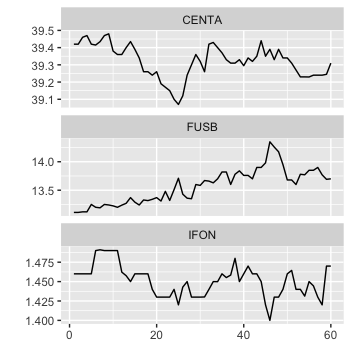
\includegraphics[width=1\linewidth, ]{Paper/images/Rplot.png}
    \caption{Plot of the closing price of some portfolio's stock}
    \label{portfolio}
\end{figure}

The choice of a 1-minute intraday time interval was purely arbitrary and it builds from the fact that with a sample of just 31 stocks the overall model can run in real time without incurring in any problem of processing time. However, in case of a bigger portfolio, a different approach may be used.

From such dataset we run the \textit{auto.arima} function and we isolated the fitting error. In order to see the goodness of fitting, we searched for autocorrelation on the residuals and we found any.

Then we built an ANN out of it which set as input the lagged stock price and as output the current error term \ref{NN_plot}.

After the model setting, we set a series of condition that creates the signal. Starting with an empty wallet we buy a stock only if our model forecast an increase in price, otherwise we don't; in case we have a stock in our wallet we'll hold it until a decrease in price is foreseen. Such condition is further highlighted in the following flowchart at figure \ref{flowchart}.


\begin{center}

\scalebox{0.4}{
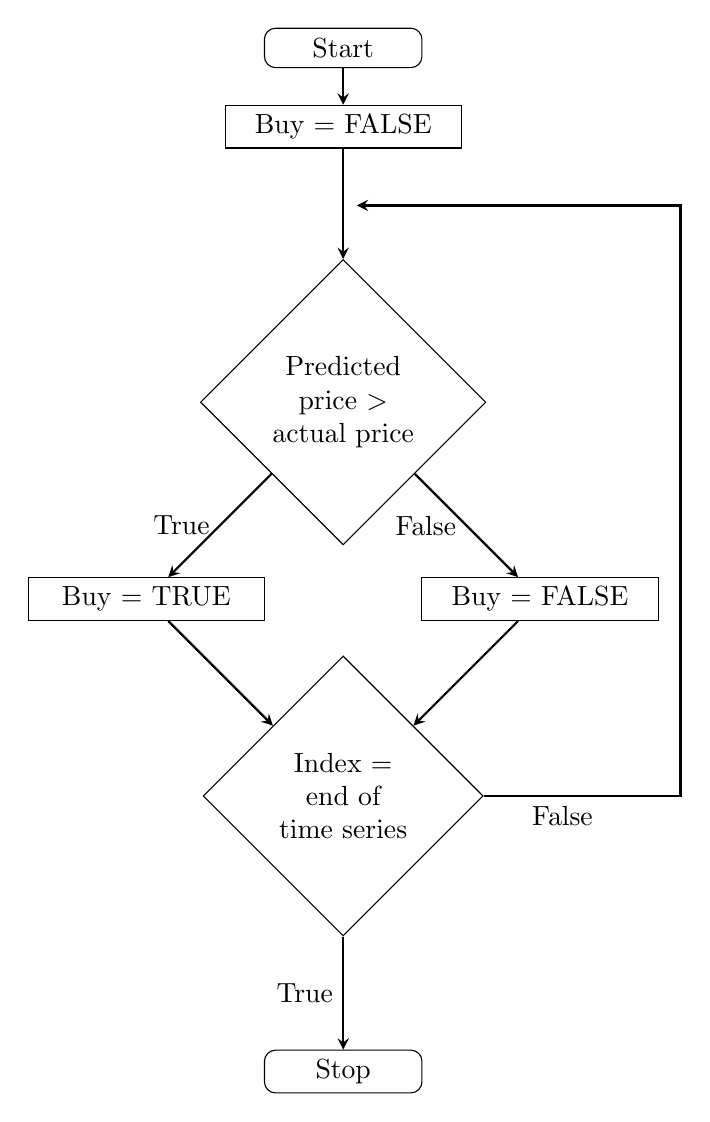
\begin{tikzpicture}

\node (start) [startstop] {Start};

\node (process1) [process, below of = start] {Buy = FALSE};

\node (blank1) [blank, below of = process1] {};

\node (d1) [decision, below of = blank1, yshift=-1.5cm]{Predicted price $>$ actual price};

\node (blank2) [blank, below of = d1, yshift=-1.5cm] {};

\node (d2) [decision, below of = blank2, yshift=-1.5cm]{Index $=$ end of time series};

\node (process2t) [process, left of = blank2, xshift=-1.5cm] {Buy = TRUE};
\node (process2f) [process, right of = blank2, xshift=1.5cm] {Buy = FALSE};

\node (stop) [startstop, below of = d2, yshift=-2.5cm] {Stop};

\draw [arrow] (start)--(process1);
\draw [arrow] (process1)--(d1);
\draw [arrow] (d1)-- node[anchor=east] {True} (process2t);
\draw [arrow] (d1)-- node[anchor=east] {False} (process2f);
\draw [arrow] (process2t)--(d2);
\draw [arrow] (process2f)--(d2);
\draw [arrow] (d2)-- node[anchor=east] {True}  (stop);
\draw [arrow] (d2.east) node[anchor=north, xshift=1cm] {False} -- ++(2.5cm,0) |- (blank1.east);

\end{tikzpicture}
}
\end{center}
  \caption{Buy and sell signal generation flowchart}
    \label{flowchart}


\section{Evidence and findings}
In the following section, we provide the results we gain from our empirical experiments, in particular, we focused on the aggregated profit and loss performed by the naive algorithm, the plain ARIMA model, and the hybrid ARIMA model. Ultimately we tested for the signal accuracy of our models computing their confusion matrixes. 
\\
After 930 rounds, that is, we run the sequence for all the stocks in the portfolio, we got the following conclusions from the model profit and loss perspective:
\begin{itemize}
    \item The hybrid model outperforms the naive algorithm;
    \item The model failed to predict in a consistent way whether the price was going up or down;
    \item Either the models alone failed to do so;
    \item The plain ARIMA performed purely in comparison with the hybrid model.
\end{itemize}

\begin{figure}
    \centering
    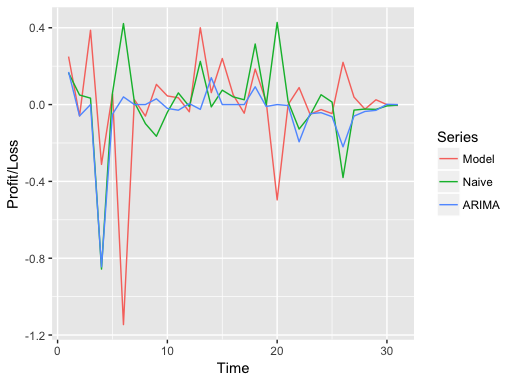
\includegraphics[width=1\linewidth, ]{Paper/images/PL_plot.png}
    \caption{Plot of the aggregate P/L per stock}
    \label{pl_portfolio}
\end{figure}

Therefore we can say that such model didn't give any competitive advantage in terms of profit and loss. However, in comparison with a plain ARIMA, the model gives a better performance but still, it's overall assessment it's not positive.

After measuring its goodness on creating profit we wanted to measure the goodness of the signal generated, and therefore its accuracy. In order to do so, we computed the confusion matrix for each model represented at figure \ref{confusionmatrix}. The main findings are reported below:
\begin{itemize}
    \item The plain ARIMA scored an accuracy of about 58,78\%; whreas
    \item The hybrid model scored value of accuracy of just 51\%;
    \item The hybrid model tend to over estimate the increase in price;
    \item The plain ARIMA instead tend to under estimate the increase in price.
\end{itemize}

\begin{figure}
    \centering
    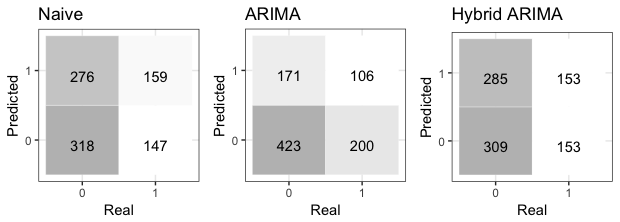
\includegraphics[width=1\linewidth, ]{Paper/images/Confusion_matrix.png}
    \caption{Confusion matrices sorted per model}
    \label{confusionmatrix}
\end{figure}

\section{Conclusion}
In this paper, we tried to apply the concept of hybrid ARIMA/ANN process as reported by Zhang in forecasting time series. We built from this model proposing an alternative in which previous information is taken into account when modeling the ANN. Such hybrid model was compared to a plain ARIMA and a naive algorithm, the process was iterated 30 times for each stock contained in a portfolio of 31 stocks from NASDAQ.
\\ 
In conclusion, we can say that the hybrid ARIMA, however, being a very interesting tool for data forecasting is still not able (at least as posed in this paper) to be used in algorithmic trading. 
\\
The writer of this article hopes that many other researchers will try to cast some light above this hybrid methodology in order to develop a better process for such modeling.

All the scripts and files are available on GitHub at the following repository:
\href{url}{https://github.com/mrepetto94/DynamicEcon} 

\newpage
\emergencystretch=1em
\sloppy

\printbibliography

\newpage
\newpage

\begin{sidewaysfigure*}[htbp]
\centering
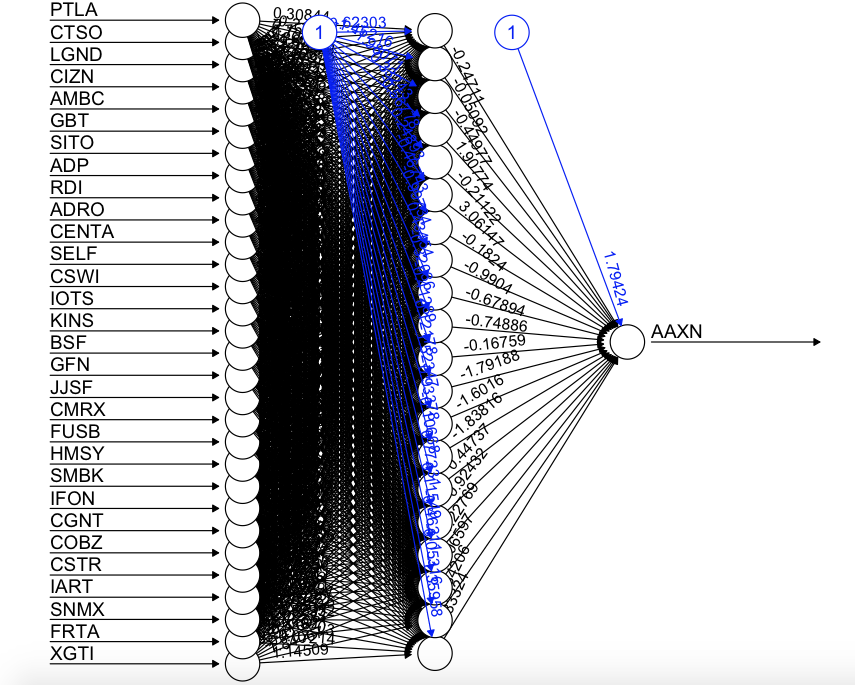
\includegraphics[width=\linewidth, height=\textheight,keepaspectratio]{Paper/images/NN_plot.png}
\caption[short]{\text{Plot of the Neural Network forecasting AAXN current errors}}
\label{NN_plot}
\end{sidewaysfigure*}

\end{document}